\documentclass[a4paper,]{article}
\usepackage{float}
\usepackage{graphicx}
\usepackage{hyperref}
\usepackage[utf8]{inputenc}
\usepackage[T2A]{fontenc}
\usepackage[english,russian]{babel}

%opening
\title{Проектирование базы данных для Социально-хозяйственного направления Студсовета}
\author{Коваленко Лев Витальевич, группа Б05-814}

\begin{document}

\maketitle{}

\pagebreak

\section{Концептуальная модель}

\Large{Cущности:}
\begin{itemize}
	\item Студент [STUDENT]
	\item Комната [ROOM]
	\item Активист [ACTIVIST]
	\item Руководитель [MANAGER]
	\item Объекты ответственности [RESPONSIBLE\_ZONE]
	\item Помещение Студсовета [ROOM\_OF\_STUDENT\_COUNCIL]
	\item Лог электронного замка [LOCK\_LOG]
	\item Бан-лист [BAN\_LIST]
\end{itemize}

\begin{figure}[H]
	\centering
	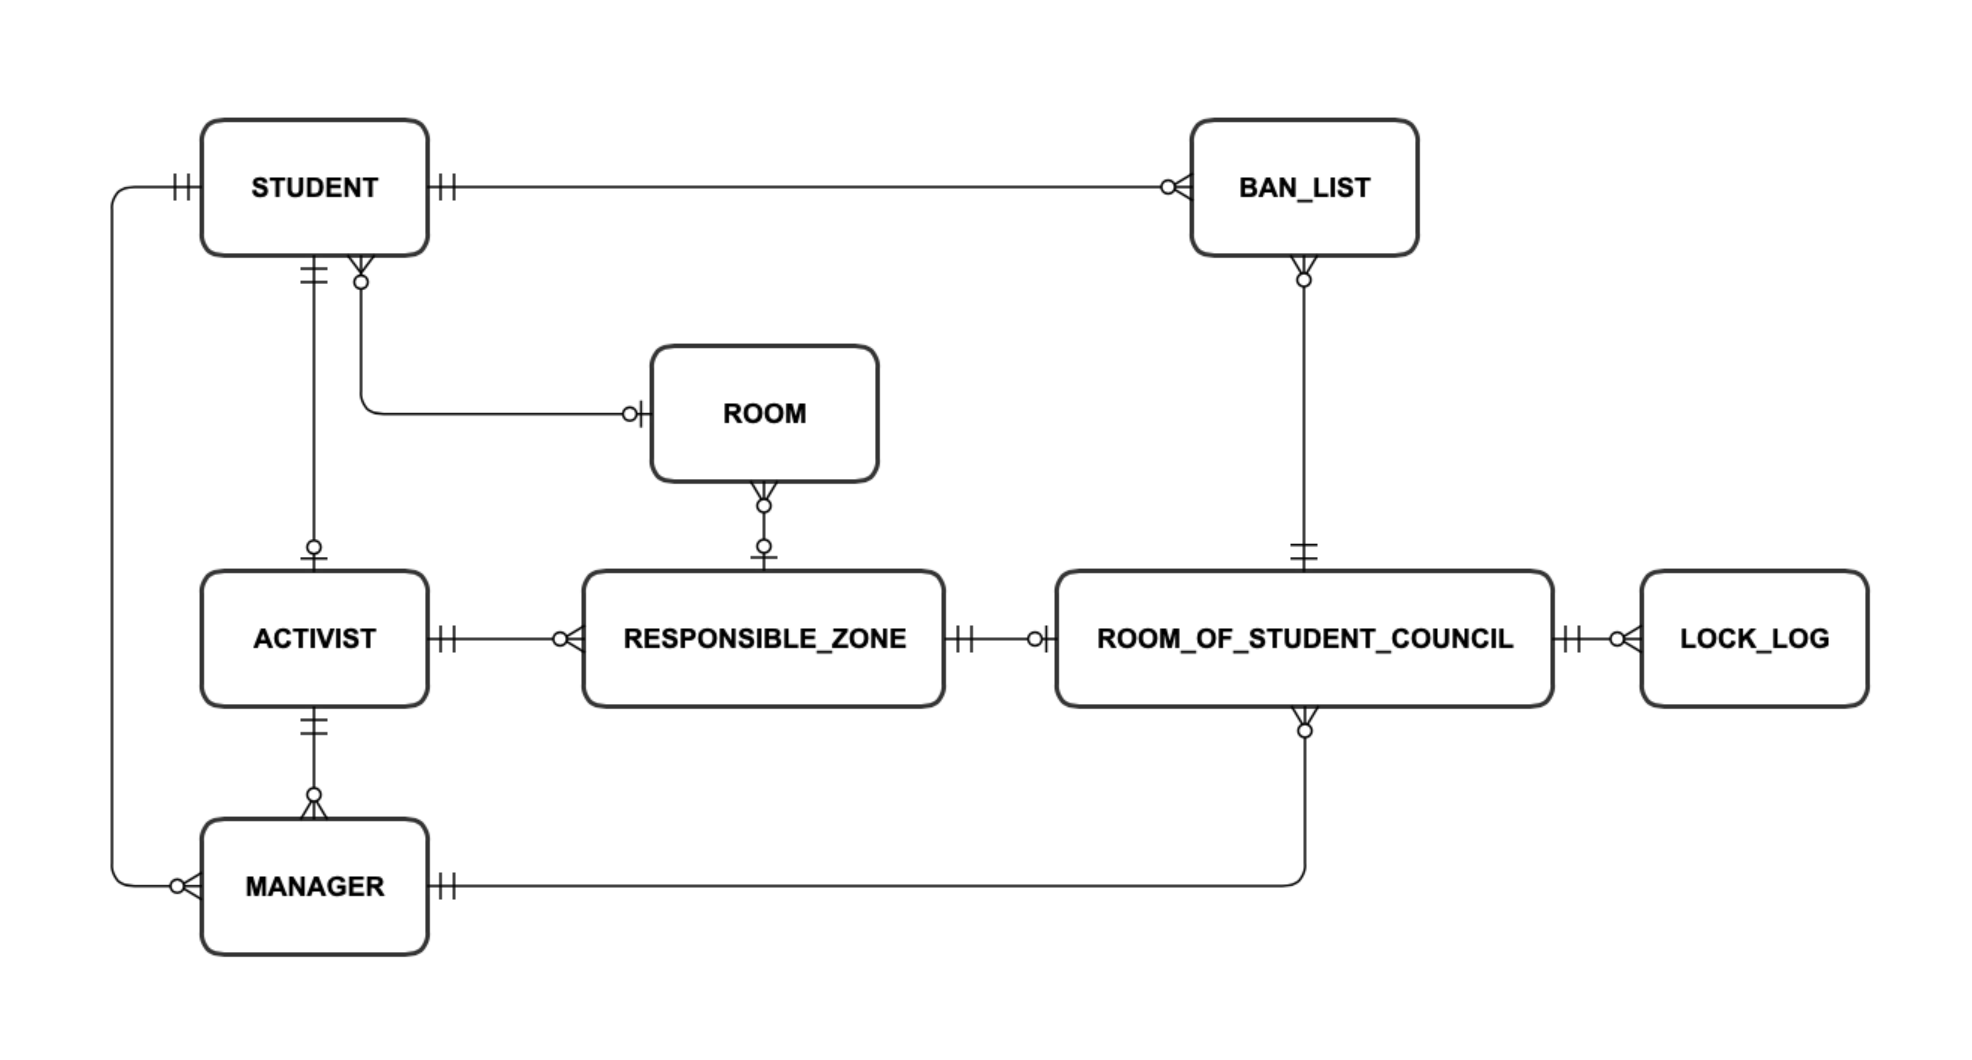
\includegraphics[height=8cm]{media/concept.png}
	\caption{Концептуальная модель}
	\label{figure:concept}
\end{figure}

\pagebreak

\section{Логическая модель}

Было принято решение создать БД, удовлетворяющую 3-ю НФ. Дублирование записей будет усложнять изменение данных, потенциально приводить к аномалиям, при том, что данные и должности меняются часто, и БД может пострадать из-за некомпетентности нового сотрудника. Размеры основных таблиц небольшие, так что это существенно не увеличит время запросов.

\begin{figure}[H]
    \centering
	\begin{center}
	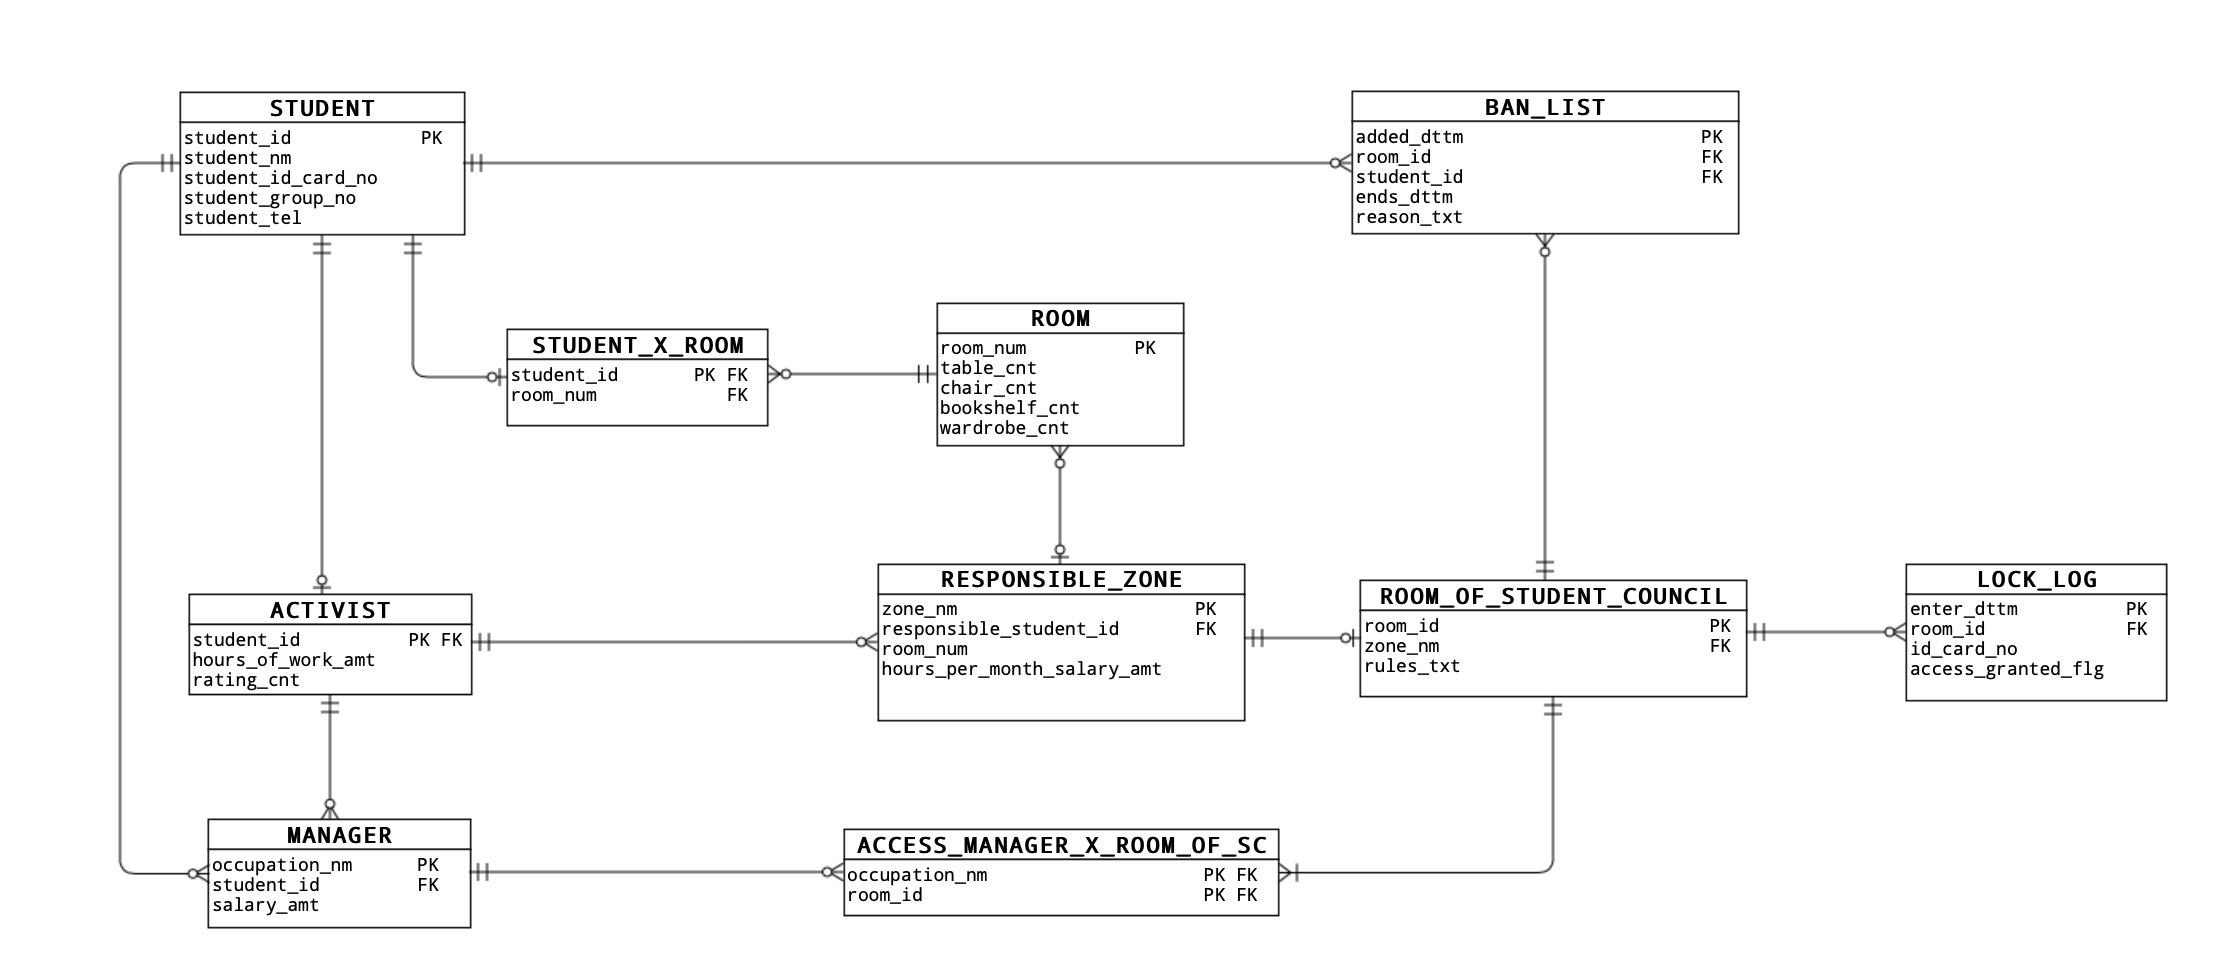
\includegraphics[width=12cm]{media/logic.jpeg}
	\caption{Логическая модель}
	\label{figure:logic}
	\end{center}
\end{figure}

\pagebreak

\section{Физическая модель}

\begin{table}[H]
    \footnotesize
	\center
	\begin{tabular}[center]{|c|p{4cm}|c|p{3cm}|}
        \hline
		Название & Описание & Тип & Ограничения \\ \hline
		student\_id & Внутренний идентификатор студента & SERIAL & PRIMARY KEY \\ \hline
		student\_nm & ФИО студента & VARCHAR(255) & NOT NULL \\ \hline
		student\_id\_card\_no & Номер пропуска студента & INT & \\ \hline
		student\_group\_no & Номер группы студента в формате Б05-814 & VARCHAR(10) &\\ \hline
		student\_tel & Телефонный номер студента без «+» & BIGINT & >=79000000000,  <=79999999999 \\ \hline
	\end{tabular}
	\caption{Студент [STUDENT]}
\end{table}

\begin{table}[H]
	\footnotesize
	\center
	\begin{tabular}[center]{|c|p{4.4cm}|c|p{2.5cm}|}
		\hline
		Название & Описание & Тип & Ограничения \\ \hline
		room\_num & Номер комнаты из трёх цифр и, возможно, 1 буквы & VARCHAR(4) & PRIMARY KEY \\ \hline
		table\_cnt & Количество письменных столов, закрепленных за комнатой & SMALLINT & NOT NULL, >=0 \\ \hline
		chair\_cnt & Количество стульев, закрепленных за комнатой & SMALLINT & NOT NULL, >=0 \\ \hline
		bookshelf\_cnt & Количество книжных полок, закрепленных за комнатой & SMALLINT & NOT NULL, >=0 \\ \hline
		wardrobe\_cnt & Количество гардеробов, закрепленных за комнатой & SMALLINT & NOT NULL, >=0 \\ \hline
	\end{tabular}
	\caption{Комната [ROOM]}
\end{table}

\begin{table}[H]
	\footnotesize
	\center
	\begin{tabular}[center]{|c|p{4cm}|c|p{3.3cm}|}
		\hline
		Название & Описание & Тип & Ограничения \\ \hline
		student\_id & Внутренний идентификатор студента & INT & PRIMARY KEY, FOREIGN KEY STUDENT (student\_id) \\ \hline
		hours\_of\_work\_amt & Часы работы активиста & DECIMAL & NOT NULL, >=0 \\ \hline
		rating\_cnt & Рейтинг активиста, показывающий его уровень (очки роста) & SMALLINT & NOT NULL, >=0 \\ \hline
	\end{tabular}
	\caption{Активист [ACTIVIST]}
\end{table}

\begin{table}[H]
	\footnotesize
	\center
	\begin{tabular}[center]{|c|p{4cm}|c|p{2.2cm}|}
		\hline
		Название & Описание & Тип & Ограничения \\ \hline
		occupation\_nm & Название должности & VARCHAR(255) & PRIMARY KEY \\ \hline
		student\_id & Внутренний идентификатор студента & INT & FOREIGN KEY STUDENT (student\_id) \\ \hline
		salary\_amt & Месячная стоимость должности (очки руководителя) & DECIMAL & >=0 \\ \hline
	\end{tabular}
	\caption{Руководитель [MANAGER]}
\end{table}

\begin{table}[H]
	\footnotesize
	\center
	\begin{tabular}[center]{|c|p{3.8cm}|c|p{3cm}|}
		\hline
		Название & Описание & Тип & Ограничения \\ \hline
		zone\_nm & Полное название объекта & VARCHAR(255) & PRIMARY KEY \\ \hline
		responsible\_student\_id & Внутренний идентификатор студента, ответственного за объект & INT & FOREIGN KEY STUDENT (student\_id) \\ \hline
		room\_num & Номер комнаты, содержащей объект или являющейся объектом & VARCHAR(4) & Не FK!! Может быть null \\ \hline
		hours\_per\_month\_salary\_amt & Месячная "зарплата"\ на должности в часах работы активиста & DECIMAL & >=0 \\ \hline
	\end{tabular}
	\caption{Объекты ответственности [RESPONSIBLE\_ZONE]}
\end{table}

\begin{table}[H]
	\footnotesize
	\center
	\begin{tabular}[center]{|c|p{4cm}|c|p{3cm}|}
		\hline
		Название & Описание & Тип & Ограничения \\ \hline
		room\_id & Идентификатор помещения (короткое название на английском без пробелов) & VARCHAR(20) & PRIMARY KEY \\ \hline
		zone\_nm & Полное название объекта & VARCHAR(255) & FK RESPONSIBLE\_ZONE (zone\_nm) \\ \hline
		rules\_txt & Правила пользования помещением & VARCHAR &  \\ \hline
	\end{tabular}
	\caption{Помещение Студсовета [ROOM\_OF\_STUDENT\_COUNCIL]}
\end{table}

\begin{table}[H]
	\footnotesize
	\center
	\begin{tabular}[center]{|c|p{4cm}|c|p{4.8cm}|}
		\hline
		Название & Описание & Тип & Ограничения \\ \hline
		enter\_dttm & Дата и время запроса входа (приложения пропуска к замку) & TIMESTAMP & PRIMARY KEY \\ \hline
		room\_id & Идентификатор помещения (короткое название на английском без пробелов) & VARCHAR(20) & FOREIGN KEY ROOM\_OF\_STUDENT\_COUNCIL (room\_id)
		 \\ \hline
		id\_card\_no & Номер пропуска, по которому была попытка входа & INT & NOT NULL, Не FK, пропуска может не быть в базе \\ \hline
		access\_granted\_flag & Был ли одобрен вход в помещение, открылась ли дверь & BOOLEAN & NOT NULL \\ \hline
	\end{tabular}
	\caption{Лог замка [LOCK\_LOG]}
\end{table}

\begin{table}[H]
	\footnotesize
	\center
	\begin{tabular}[center]{|c|p{4cm}|c|p{4.8cm}|}
		\hline
		Название & Описание & Тип & Ограничения \\ \hline
		added\_dttm & Дата и время добавления блокировки & TIMESTAMP & PRIMARY KEY \\ \hline
		room\_id & Идентификатор помещения (короткое название на английском без пробелов) & VARCHAR(20) & FOREIGN KEY ROOM\_OF\_STUDENT\_COUNCIL (room\_id)
		 \\ \hline
		student\_id & Внутренний идентификатор заблокированного студента & INT & FOREIGN KEY STUDENT (student\_id) \\ \hline
		ends\_dttm & Дата и время окончания блокировки & TIMESTAMP & NOT NULL \\ \hline
		reason\_txt & Причина блокировки & VARCHAR &  \\ \hline
	\end{tabular}
	\caption{Бан-лист в помещения Студсовета [BAN\_LIST]}
\end{table}

\begin{table}[H]
	\footnotesize
	\center
	\begin{tabular}[center]{|c|p{4cm}|c|p{3cm}|}
		\hline
		Название & Описание & Тип & Ограничения \\ \hline
		student\_id & Внутренний идентификатор студента & INT & PRIMARY KEY, FOREIGN KEY STUDENT (student\_id) \\ \hline
		room\_num & Номер комнаты из трёх цифр и, возможно, 1 буквы & VARCHAR(4) & FOREIGN KEY ROOM (room\_num) \\ \hline
	\end{tabular}
	\caption{Таблица связи проживания Студент - Комната [STUDENT\_X\_ROOM]}
\end{table}

\begin{table}[H]
	\footnotesize
	\center
	\begin{tabular}[center]{|c|p{4cm}|c|p{5cm}|}
		\hline
		Название & Описание & Тип & Ограничения \\ \hline
		occupation\_nm & Название должности & VARCHAR(255) & PRIMARY KEY, FOREIGN KEY MANAGER (occupation\_nm) \\ \hline
		room\_id & Идентификатор помещения (короткое название на английском без пробелов) & VARCHAR(20) & PRIMARY KEY, FOREIGN KEY ROOM\_OF\_STUDENT\_COUNCIL (room\_id) \\ \hline

	\end{tabular}
	\caption{Таблица связи доступа по должности Руководитель – Помещение Студсовета [ACCESS\_MANAGER\_X\_ROOM\_OF\_SC]}
\end{table}



\end{document}
